\chapter{Introduktionsopgaver}
Som kort beskrevet i Introduktionen begyndte vi dette projekt med at lave en række opgaver, både håndregningsopgaver og en del programmeringsopgaver.

\section{Håndregningsopgaver}
Vores besvarelser af håndregningsopgaverne omhandlende bit- og hexadecimalmanipulation kan ses på figur \ref{fig: Ex1.1}, figur \ref{fig: Ex2.1}, figur \ref{fig: Ex3.1} og figur \ref{fig: Ex4.4}.\\ \\


\begin{figure}[h!]
\centering
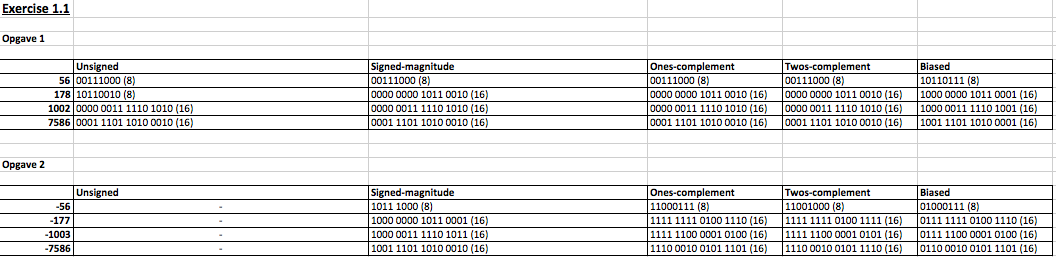
\includegraphics[scale=0.4]{figs/Ex1.png}
\caption{Vores besvarelse af Exercise 1.1}
\label{fig:Ex1.1}
\end{figure}

\begin{figure}[h!]
\centering
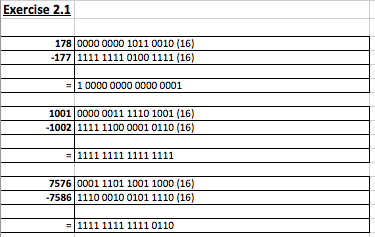
\includegraphics[scale=0.6]{figs/Ex2.png}
\caption{Vores besvarelse af Exercise 2.1}
\label{fig:Ex2.1}
\end{figure}

\begin{figure}[h!]
\centering
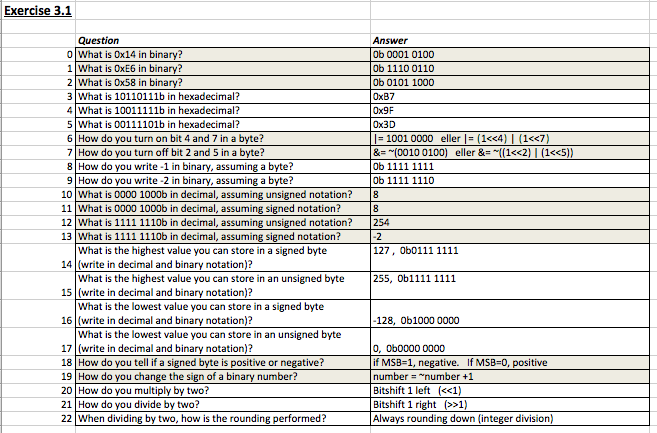
\includegraphics[scale=0.6]{figs/Ex3.png}
\caption{Vores besvarelse af Exercise 3.1}
\label{fig:Ex3.1}
\end{figure}

\begin{figure}[h!]
\centering
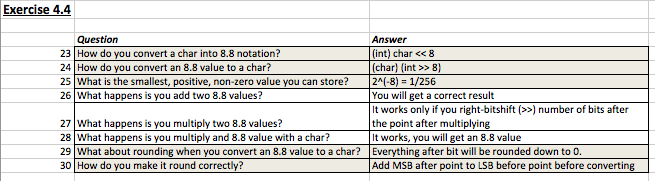
\includegraphics[scale=0.6]{figs/Ex4.png}
\caption{Vores besvarelse af Exercise 4.4}
\label{fig:Ex4.4}
\end{figure}

\section{Programmeringsopgaver}
En del af de programmer vi skrev under introforløbet endte vi med at bruge i ReflexBall-spillet i modificerede versioner. Disse inkluderer \nameref{ansi}, \nameref{charset}, \nameref{buttons}, \nameref{LED}, \nameref{lut}, \nameref{math} og \nameref{time} og kan ses i \textbf{Appendiks C} i deres modificerede versioner. I \textbf{Appendiks C} er der fjernet noget af det oprindelige kode i \nameref{ansi} og i \nameref{time}, hvilket skyldes at vi ikke brugte de givne funktioner i implementeringen af Reflex Ball.